\documentclass[a4paper,10pt]{article}
\usepackage[english]{babel}
\usepackage{amsmath,amsfonts,amsthm}
\usepackage[utf8]{inputenc}
\usepackage{enumitem}
\usepackage{bm}
\usepackage{tikz}
\usepackage{microtype}
\usepackage[bf,hang,small]{caption}
\usepackage[colorlinks=true, linkcolor=black, citecolor=black, filecolor=black, menucolor=black, urlcolor=black]{hyperref}
\usepackage{natbib}
\setcitestyle{numbers,square,citesep={,}}

\graphicspath{{./}{graphics/}}


\title{Unnamed Project for Computing Persistent Homology With Haskell}
\author{Gard Spreemann}
\date{\today}

\begin{document}
\maketitle

\section*{Caveats}
First of all, my Haskell-fu is weak. I surely make many mistakes,
ranging from the cute ones that invite \emph{oh, that's nice, but that
  ten-line function you wrote is really just the following cryptic
  composition of six built-in functions with scary names} from more
skilled people, to horrible designs and performance problems.

More importantly, there may very well be serious mistakes in my code
that have nothing to do with Haskell. I will not guarantee that my
code will leave your house intact or your pets alive, let alone that
it will actually correctly compute persistent homology of your point
cloud! I have done some sanity checks against
javaPlex~\citep{javaplex}, but these are far from exhaustive. Beware.

To conclude, the Unnamed Project for Persistent Homology in Haskell
(hereafter ``pershom'') is not at all something I feel is ready to be
shared with the world. However, after Mikael Vejdemo Johansson made me
aware that he and Andrew Tausz have been working on their own Haskell
persistent homology project, hPlex~\citep{hplex}, I concluded that
maybe there would be some slight use for my horrible code
afterall. Better to swallow my pride than to run the risk of others
having to redo my work.

\section{Overview}
When designing pershom, I've tried to mimic the ``philosophy''
outlined in \citep{compph,fcvr} (as I see it, at least): From a point
cloud arises a neighborhood graph, from which one computes a
Vietoris--Rips complex. From a Vietoris--Rips complex, or indeed any
suitable filtered complex, one computes persistent homology. This
calls for a natural modularization of the code corresponding to the
distinct phases outlined by the process.

Hopefully, this modularization will make it easier to implement many
different algorithms at the various stages: Many ways to compute the
neighborhood graph, many ways to generate a filtered complex from it,
and different ways to compute the persistent homology of the
latter. Currently though, it's all pretty shallow:
\begin{enumerate}[label=\arabic*)]
  \item Brute-force computation of neighborhood graphs is implemented
    in the \texttt{NeighborhoodGraph} module. The function
    \texttt{exact :: (Metric a) => Cloud a -> Double ->
      NeighborhoodGraph} computes the exact neighborhood graph of the
    supplied point cloud up to a maximum scale (as described
    in~\citep{fcvr}).
  \item The module \texttt{VietorisRips} implements ``the inductive
    algorithm'' of~\citep{fcvr}. The function \texttt{inductive :: Int
      -> NeighborhoodGraph -> VietorisRips} expands a neighborhood
    graph into a Vietoris--Rips complex. To be precise,
    \texttt{inductive d g} computes the $d$-skeleton of the
    neighborhood graph \texttt{g}. In the same module,
    \texttt{filtration :: VietorisRips -> [Double] -> FilteredComplex
      Double Int} turns the Vietoris--Rips data structure into one
    made for filtered complexes in general. The \texttt{Int}
    parameterizing \texttt{FilteredComplex} refers to the datatype
    used for vertices in the simplices.
  \item Finally, the module \texttt{PersistentHomology}, specifically
    the function \texttt{persistentHomology :: (Ord a, Field b) =>
      FilteredComplex c a -> PersistentHomology a b} computes the
    persistent homology of a filtered complex. Computation is done
    over the field \texttt{b}. The module also includes facilities
    conversion into barcodes.
\end{enumerate}

\subsection{How to use}
Documentation is seriously lacking, but hopefully one can learn
something from looking at two example programs located in the
\texttt{test} directory. \texttt{TestVR} reads a point cloud from
standard input and computes the Vietoris--Rips complex of it, while
\texttt{TestPH} computes persistent homology.

I have not yet Cabalized pershom, so these programs must be compiled
with for example \texttt{ghc -i../.. -O2 --make TestVR.hs -o testvr}.

\texttt{test} and its subdirectories also contain a few crude Python
utilities to generate point clouds and plot barcodes and 2D
Vietoris--Rips complexes. There are also small Java programs that use
javaPlex for comparison with pershom.

\subsection{Requirements}
The current version of pershom has only been tested with GHC
7.0.3. Apart from \texttt{base}, I'm quite sure the only package
needed is \texttt{vector} (I've only tried version 0.7.0.1).

The Python utilities need Python, Numpy, SciPy and Matplotlib. The
javaPlex test programs naturally need Java and javaPlex (tested with
version 4).

\section{Known problems}
\begin{itemize}
  \item There are severe performance problems in
    \texttt{PersistentHomology}. The data structure used, a
    \texttt{Data.Map}, is not suitable in the long run, and profiling
    reveals (to no surprise) that a lot of time is spent calling
    \texttt{maxSimplex}, which involves comparing simplices based on
    their order in the persistent homology data structure. I am aware
    of this, but have not had time to rethink it.
  \item Generation of the Vietoris--Rips complex has been tested quite
    a bit against the output of javaPlex, and found to match. The
    birth/death of generators in persistent homology, though, are
    often off by one. This has not been investigated fully.
  \item The amount of unknown problems that are very likely to exist.
\end{itemize}

\section{To do}
Obviously, the project is severely lacking in many ways. Below is a
list with ideas for the future.
\begin{itemize}
  \item The persistent homology and barcode structures operate with
    filtration levels instead of values. This should perhaps change.
  \item There is room for parallelization at the neighborhood graph
    and Vietoris--Rips expansion stages.
  \item Performance of the persistent homology calculations must be
    improved.
  \item Witness complex.
  \item Complete Haddock markup and documentation.
  \item More QuickCheck testcases.
  \item Cabalization.
  \item Reordering the modules into a proper hierarchy.
  \item $\dots$
\end{itemize}

\section{Stuff}
A sanity check based on the javaPlex tutorial's torus
example~\citep{javaplextut} follows. Sadly, this is one of the cases
in which javaPlex outperforms pershom by about an order of
magnitude. The test program was run with \texttt{testph -s 0.9 -d 3
  -N 100 < points.txt > out.txt}, where \texttt{points.txt} was
generated with \texttt{generate-torus.py}. See
figures~\ref{fig:torus0}--\ref{fig:torus2}.

\begin{figure}[htpb]
  \centering
  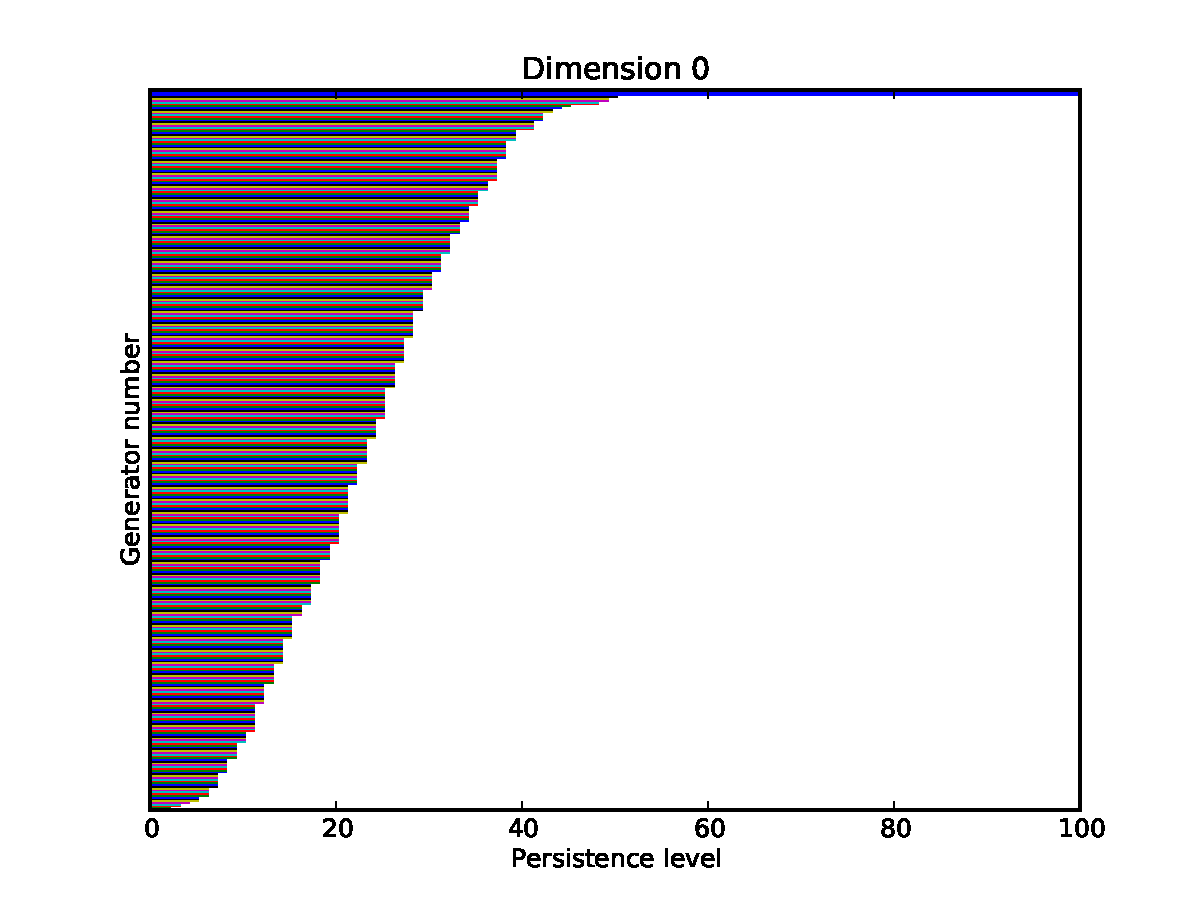
\includegraphics[width=0.9\textwidth]{torus_d0}
  \caption{The $0$-dimensional persistent homology of $400$ points uniformly sampled from a unit torus, as in~\citep{javaplextut}. The maximum persistence level is $0.9$.} \label{fig:torus0}
\end{figure}
\begin{figure}[htpb]
  \centering
  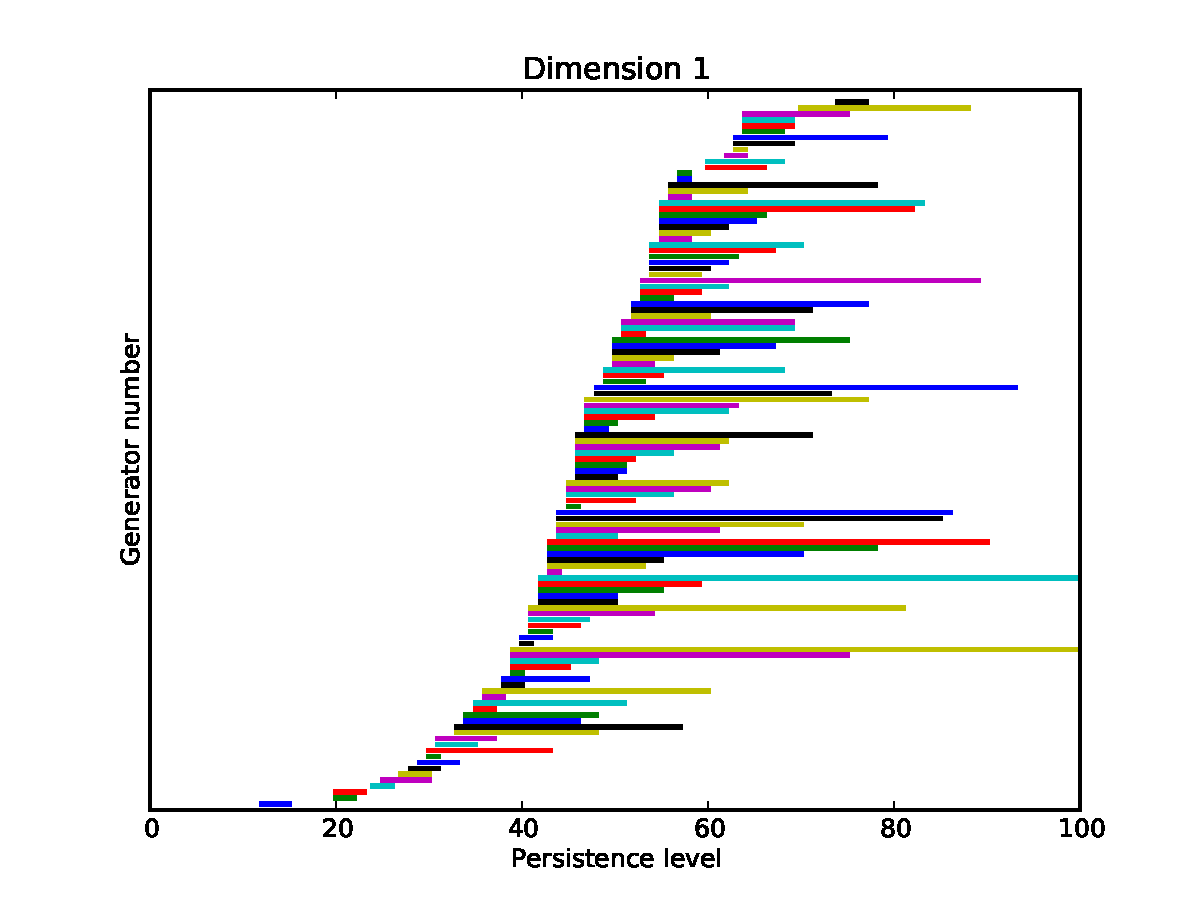
\includegraphics[width=0.9\textwidth]{torus_d1}
  \caption{The $1$-dimensional persistent homology of $400$ points uniformly sampled from a unit torus, as in~\citep{javaplextut}. The maximum persistence level is $0.9$.} \label{fig:torus1}
\end{figure}
\begin{figure}[htpb]
  \centering
  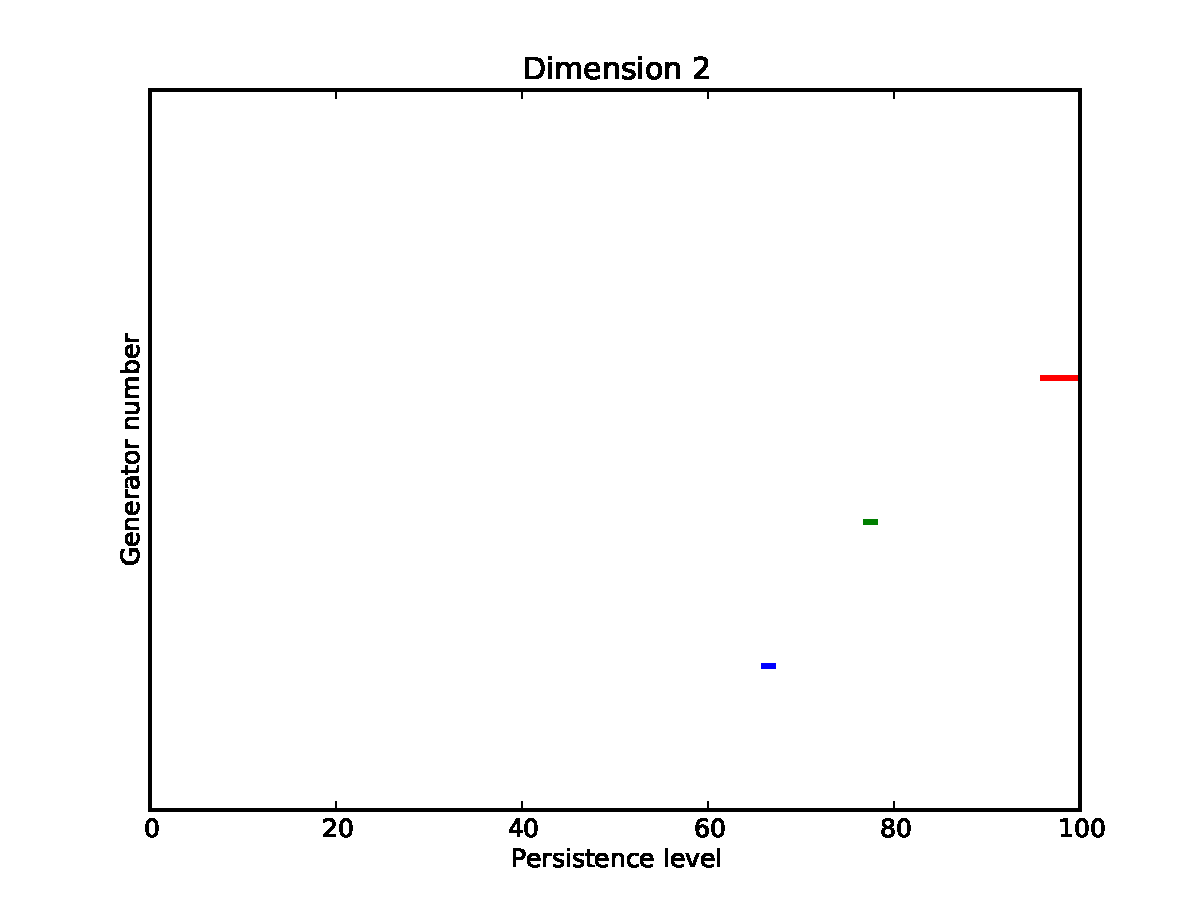
\includegraphics[width=0.9\textwidth]{torus_d2}
  \caption{The $2$-dimensional persistent homology of $400$ points uniformly sampled from a unit torus, as in~\citep{javaplextut}. The maximum persistence level is $0.9$.} \label{fig:torus2}
\end{figure}

\bibliography{pershom}
\bibliographystyle{amsplain}
\end{document}
